\documentclass[UTF8,a4paper,12pt]{ctexart}

\usepackage[a4paper,left=2.4cm,right=2.4cm,top=2.6cm,bottom=2.6cm]{geometry}
\usepackage{graphicx}
\usepackage{booktabs}
\usepackage{array}
\usepackage{float}
\usepackage{caption}
\usepackage{subcaption}
\usepackage{amsmath}
\usepackage{amssymb}
\usepackage{hyperref}
\usepackage{enumitem}
\usepackage{xcolor}
\usepackage{listings}
\usepackage{longtable}
\usepackage{multirow}
\usepackage{fancyhdr}
\usepackage{lastpage}
\usepackage{titlesec}

\hypersetup{hidelinks}
\graphicspath{{./}{fig/}}
\captionsetup{font=small}

\pagestyle{fancy}
\setlength{\headheight}{15pt}
\fancyhf{}
\lhead{并行程序设计实验报告}
\rhead{CPU架构相关编程}
\cfoot{\thepage/\pageref{LastPage}}

\setcounter{secnumdepth}{3}
\setcounter{tocdepth}{3}
\renewcommand{\contentsname}{目录}
\renewcommand{\thesection}{\chinese{section}、}
\renewcommand{\thesubsection}{（\chinese{subsection}）}
\renewcommand{\thesubsubsection}{\arabic{subsubsection}.}
\titleformat{\section}{\Large\bfseries}{\thesection}{0.5em}{}
\titleformat{\subsection}{\large\bfseries}{\thesubsection}{0.5em}{}
\titleformat{\subsubsection}{\normalsize\bfseries}{\thesubsubsection}{0.5em}{}
\titlespacing*{\section}{0pt}{1.2em}{0.6em}
\titlespacing*{\subsection}{0pt}{0.9em}{0.4em}
\titlespacing*{\subsubsection}{0pt}{0.7em}{0.3em}

\lstset{
  language=C++,
  basicstyle=\ttfamily\fontsize{8.2pt}{9.0pt}\selectfont,
  keywordstyle=\color{blue!70!black}\bfseries,
  commentstyle=\color{green!40!black},
  stringstyle=\color{orange!60!black},
  numbers=left,
  numberstyle=\fontsize{7pt}{7pt}\selectfont,
  stepnumber=1,
  numbersep=6pt,
  frame=single,
  captionpos=b,
  breaklines=true,
  tabsize=4,
  aboveskip=4pt,
  belowskip=4pt,
  showstringspaces=false
}

\newcommand{\placeholder}[1]{%
  \begin{center}
  \fbox{\parbox[c][4.4cm][c]{0.9\textwidth}{\centering #1}}
  \end{center}}

\begin{document}

\begin{titlepage}
    \centering
    
\includegraphics[width=0.22\textwidth]{NKU.png}\\[1.2cm]
    {\heiti\zihao{2} 计算机学院\\[0.5cm]}
    {\heiti\zihao{2} 并行程序设计实验报告\\[2.0cm]}
    {\heiti\zihao{0} CPU架构相关编程\\[2.6cm]}

    \renewcommand{\arraystretch}{1.6}
    \begin{tabular}{>{\raggedleft\arraybackslash}p{4cm} p{8cm}}
        姓名： & 崔迪 \\
        学号： & 2412439 \\
        专业： & 计算机科学与技术 \\
        课程： & 并行程序设计 \\
        指导教师： & 崔立骁 \\
        完成日期： & \today \\
    \end{tabular}

    \vfill
\end{titlepage}

\tableofcontents
\clearpage

\section*{摘要}
本实验围绕 CPU 架构相关编程中的两个基础问题展开：一是 \(n\times n\) 矩阵与向量内积，二是 \(n\) 个数求和。针对矩阵与向量内积，分别实现了按列访问的平凡算法和按行访问的 cache 优化算法；针对求和问题，分别实现了链式累加、两路链式累加以及两两相加的递归算法三种实现。实验采用固定数据构造方式，以高精度计时器对不同问题规模下的程序平均运行时间进行测量，并将结果导出为 CSV 文件后进一步绘图分析。

实验结果表明：对于矩阵与向量内积问题，若按实验平台信息中给出的 cache 容量选择“未充满 L1、未充满 L2、未充满 L3、基本充满 L3、溢出 L3”五个阶段的规模，按行访问的 cache 优化算法始终优于按列访问的平凡算法；当矩阵规模增至 \(n=2048\)（32 MiB，已明显超过 24 MiB 的 L3）时，相较平凡算法获得约 23.00 倍加速。对于 \(n\) 个数求和问题，两路链式累加始终优于平凡链式累加，说明减少累加依赖链长度、提升指令级并行能力是有效的。递归算法虽然在理论上具有更短的依赖深度，但在当前单线程实现中由于存在额外复制和多轮中间结果写回，其实际性能未超过两路链式累加。进阶部分进一步给出了循环展开优化的设计思路，并为后续的性能测试与 profiling 留出了补充位置。

本次实验的代码和结果均在\url{https://github.com/changluei/Parallel-Programming}
\section*{实验平台信息}
\begin{table}[H]
    \centering
    \begin{tabular}{>{\raggedright\arraybackslash}p{4cm} p{10cm}}
        \toprule
        项目 & 说明 \\
        \midrule
        操作系统 & Microsoft Windows 11 家庭中文版（10.0.26200） \\
        处理器 & 13th Gen Intel(R) Core(TM) i7-13650HX，14 核 20 线程，最高时钟频率 2.60 GHz \\
        CPU各级cache & L1:1.2 MB\hspace{2.5em}L2:11.5 MB\hspace{2.5em}L3:24.0 MB \\
        内存 & 13.70 GiB \\
        编译器 & \texttt{g++}（MinGW），主要编译选项为 \texttt{-O2 -std=c++17} \\
        绘图环境 & Conda 环境 \texttt{parallel}，Python 配合 \texttt{matplotlib}、\texttt{pandas}、\texttt{numpy} \\
        profiling 工具 & Intel VTune Profiler 2025.10 \\
        数据组织 & 原始实验数据以 CSV 文件形式保存在 \texttt{results} 目录中，绘图结果保存在 \texttt{fig} 目录中 \\
        \bottomrule
    \end{tabular}
\end{table}

\clearpage
\section{基础要求}

\subsection{算法设计}

\subsubsection{\(n*n\) 矩阵与向量内积}
设输入向量为 \(a\in\mathbb{R}^{n}\)，矩阵为 \(B\in\mathbb{R}^{n\times n}\)，输出向量为 \(c\in\mathbb{R}^{n}\)。本实验计算矩阵每一列与向量 \(a\) 的内积，即
\[
    c_j = \sum_{i=0}^{n-1} B_{i,j}a_i,\qquad j=0,1,\ldots,n-1.
\]

本实验实现了两种算法。
\begin{enumerate}[label=\arabic*.]
    \item \textbf{平凡算法（逐列访问）}：外层循环按列遍历，内层循环按行累加，即访问顺序为 \texttt{B[row * n + col]}。由于矩阵在内存中按行连续存放，这种按列跨步访问会频繁跨越 cache line，属于 cache 不友好的访问方式。
    \item \textbf{cache 优化算法（逐行访问）}：先将结果向量清零，然后按行遍历矩阵，将当前行的每个元素与对应的 \(a[row]\) 相乘并直接累加到结果向量中。该实现与矩阵的行主序存储方式一致，内层循环访问连续内存，更利于 cache 预取与空间局部性利用。
\end{enumerate}

两种算法的数学结果等价，但由于访存模式不同，在现代处理器上会表现出明显不同的运行时间与 cache 行为。

\subsubsection{\(n\) 个数求和}
对于数组 \(x[0],x[1],\ldots,x[n-1]\)，目标是计算
\[
    S = \sum_{i=0}^{n-1} x[i].
\]
本实验实现了以下三种求和方式。
\begin{enumerate}[label=\arabic*.]
    \item \textbf{平凡算法（链式累加）}：维护单个累加器 \texttt{sum}，按顺序执行 \texttt{sum += x[i]}。该方法实现最简单，但加法之间形成一条很长的数据依赖链。
    \item \textbf{优化算法（两路链式累加）}：维护两个独立累加器 \texttt{sum1} 和 \texttt{sum2}，分别累加奇偶位置，循环结束后再合并两个部分和。该方法可以打断单一依赖链，更有利于超标量处理器挖掘指令级并行。
    \item \textbf{递归思想（两两相加）}：先将相邻两个元素相加得到 \(n/2\) 个中间结果，再对中间结果继续两两相加，重复进行 \(\log_2 n\) 轮，直到剩下一个结果。本次实验采用二重循环方式实现。
\end{enumerate}

其中，两路链式累加和递归思想都属于对处理器执行特性的利用：前者重点减少串行依赖、增强指令级并行，后者则从规约树结构上缩短依赖深度。
\subsection{编程实现}

\subsubsection{\(n*n\) 矩阵与向量内积}
为了便于实验比较，程序使用固定规则自动生成输入向量和矩阵，为便于测量不同规模的数据，本次采用\texttt{vector}实现。由于篇幅限制原因，本次不再展示平凡算法的实现。

\begin{lstlisting}[caption={矩阵与向量内积的优化算法核心实现}]
//优化算法实现
fill(sum.begin(), sum.end(), 0.0);
for (int row = 0; row < n; ++row) {//逐行访问矩阵元素
    const double factor = a[row];
    const size_t offset = static_cast<size_t>(row) * n;
    for (int col = 0; col < n; ++col) {
        sum[col] += b[offset + col] * factor;
    }
}

\end{lstlisting}

\subsubsection{\(n\) 个数求和}
本次同样采用固定规则生成数据。其核心求和代码如下。

\begin{lstlisting}[caption={两种求和优化核心实现}]
//两路链式累加实现
double sum1 = 0.0;double sum2 = 0.0;int i = 0;
const int n = static_cast<int>(data.size());
for (; i + 1 < n; i += 2) {
    sum1 += data[i];
    sum2 += data[i + 1];
}
for (; i < n; ++i) {
    sum1 += data[i];
}
return sum1 + sum2;
//两两相加的递归算法实现，采用二重循环实现
copy(input.begin(), input.end(), work.begin());
for (int m = static_cast<int>(input.size()); m > 1; m /= 2) {
    for (int i = 0; i < m / 2; ++i) {
        work[i] = work[i * 2] + work[i * 2 + 1];
    }
}
return work[0];

\end{lstlisting}

\subsection{性能测试}

\subsubsection{\(n*n\) 矩阵与向量内积}

本实验采用 \texttt{chrono::steady\_clock} 作为计时工具，对各算法的核心计算部分进行高精度计时。\texttt{steady\_clock} 具有单调递增、不受系统时间调整影响的特点，适合用于性能测试。测试时将算法主体封装为独立函数，在主程序中对同一规模下的算法重复执行多次，并以总耗时除以重复次数得到平均运行时间 \texttt{avg\_ms}，从而减小单次测量误差带来的影响。
矩阵实验不再采用简单倍增的规模序列，而是按照实验平台表中给出的 L1=1.2 MiB、L2=11.5 MiB、L3=24.0 MiB 选点，以观察“未充满 L1、未充满 L2、未充满 L3、基本充满 L3、溢出 L3”五个阶段的性能变化。综合“尽量采用$ 2^n $的幂规模”和“需要覆盖不同 cache 阶段”两点考虑，最终选取 \(n=256,1024,1536,1792,2048\)，对应矩阵大小分别约为 0.50 MiB、8.00 MiB、18.00 MiB、24.50 MiB 和 32.00 MiB。由于不同规模下的运行时间差异较大，重复次数分别设置为 4000、500、250、150 和 100。实验结果如图 \ref{fig:matrix-runtime} 所示，详细数据见表 \ref{tab:matrix-runtime}。

\begin{table}[H]
    \centering
    \begin{tabular}{ccccc}
        \toprule
        规模 \(n\) & 矩阵大小（MiB） & 平凡算法（ms） & cache 优化算法（ms） & 加速比 \\
        \midrule
        256   & 0.50    & 0.032270   & 0.020948   & 1.54 \\
        1024  & 8.00    & 3.844896   & 0.310954   & 12.36 \\
        1536  & 18.00   & 11.484792  & 1.481136   & 7.75 \\
        1792  & 24.50   & 15.754887  & 1.888080   & 8.34 \\
        2048  & 32.00   & 53.424360  & 2.322430   & 23.00 \\
        \bottomrule
    \end{tabular}
    \caption{矩阵与向量内积性能测试结果}
    \label{tab:matrix-runtime}
\end{table}

\begin{figure}[H]
    \centering
    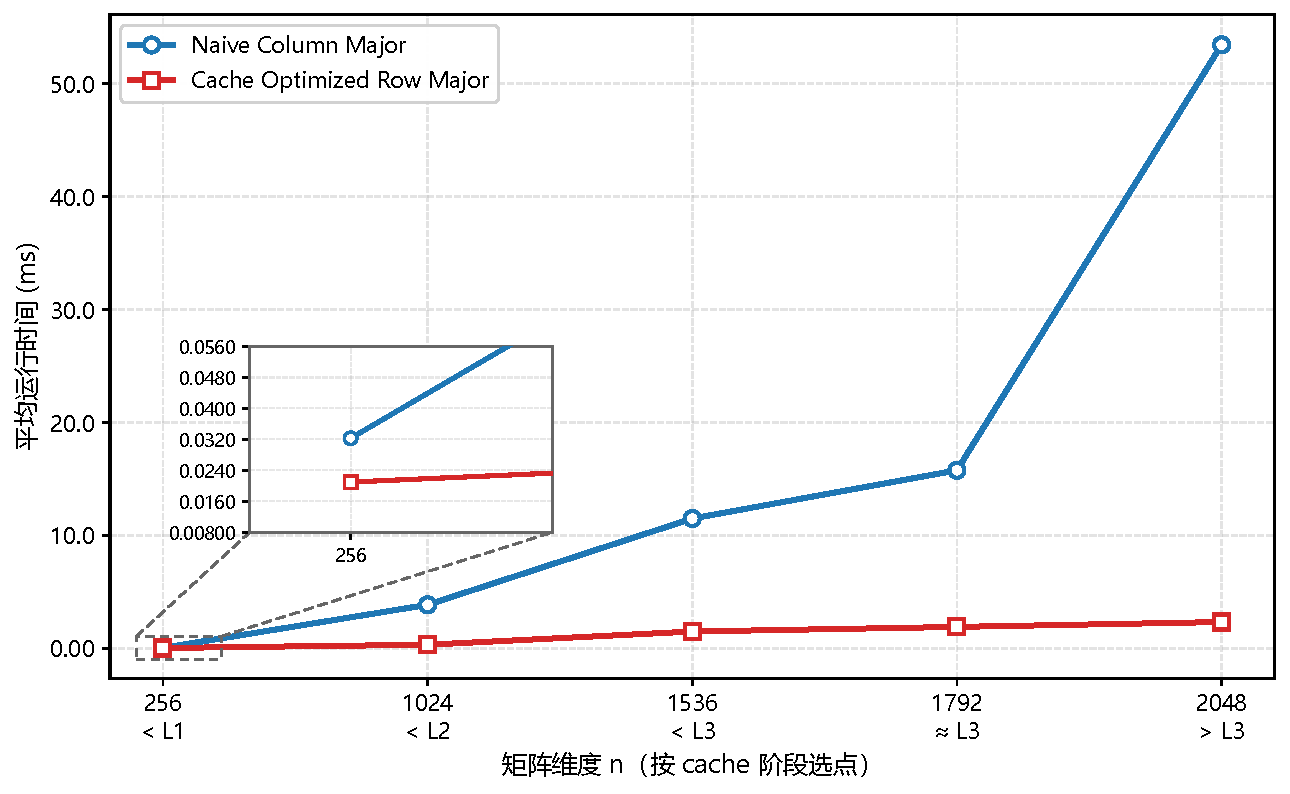
\includegraphics[width=0.88\textwidth]{fig/matrix_vector_dot_runtime_curve.pdf}
    \caption{矩阵与向量内积运行时间折线图}
    \label{fig:matrix-runtime}
\end{figure}

从图中可以看到，按 cache 阶段选点后，矩阵规模从未充满 L1 逐步增大到溢出 L3 时，平凡算法与 cache 优化算法之间的差距整体上明显拉大，尤其在 24 MiB 附近继续增大到 32 MiB 时出现了更显著的性能跳升。相关具体分析将会在后文展开。

\subsubsection{\(n\) 个数求和}
求和实验选择规模 \(n=2^{10},2^{11},2^{12},2^{13},2^{14}\)，即 1024 到 16384。由于单次求和耗时极短，为了提高计时稳定性，每个数据点均重复执行 1000 次并取平均值。实验结果如图 \ref{fig:sum-runtime} 和表 \ref{tab:sum-runtime} 所示。

\begin{table}[H]
    \centering
    \begin{tabular}{cccccc}
        \toprule
        规模 \(n\) & 平凡链式（ms） & 两路链式（ms） & 递归算法（ms） & 平凡/两路 & 平凡/递归 \\
        \midrule
        1024  & 0.000411 & 0.000214 & 0.000345 & 1.92 & 1.19 \\
        2048  & 0.000890 & 0.000452 & 0.000587 & 1.97 & 1.52 \\
        4096  & 0.001754 & 0.000855 & 0.001323 & 2.05 & 1.33 \\
        8192  & 0.003638 & 0.001730 & 0.003193 & 2.10 & 1.14 \\
        16384 & 0.007332 & 0.003606 & 0.006953 & 2.03 & 1.05 \\
        \bottomrule
    \end{tabular}
    \caption{\(n\) 个数求和性能测试结果}
    \label{tab:sum-runtime}
\end{table}

\begin{figure}[H]
    \centering
    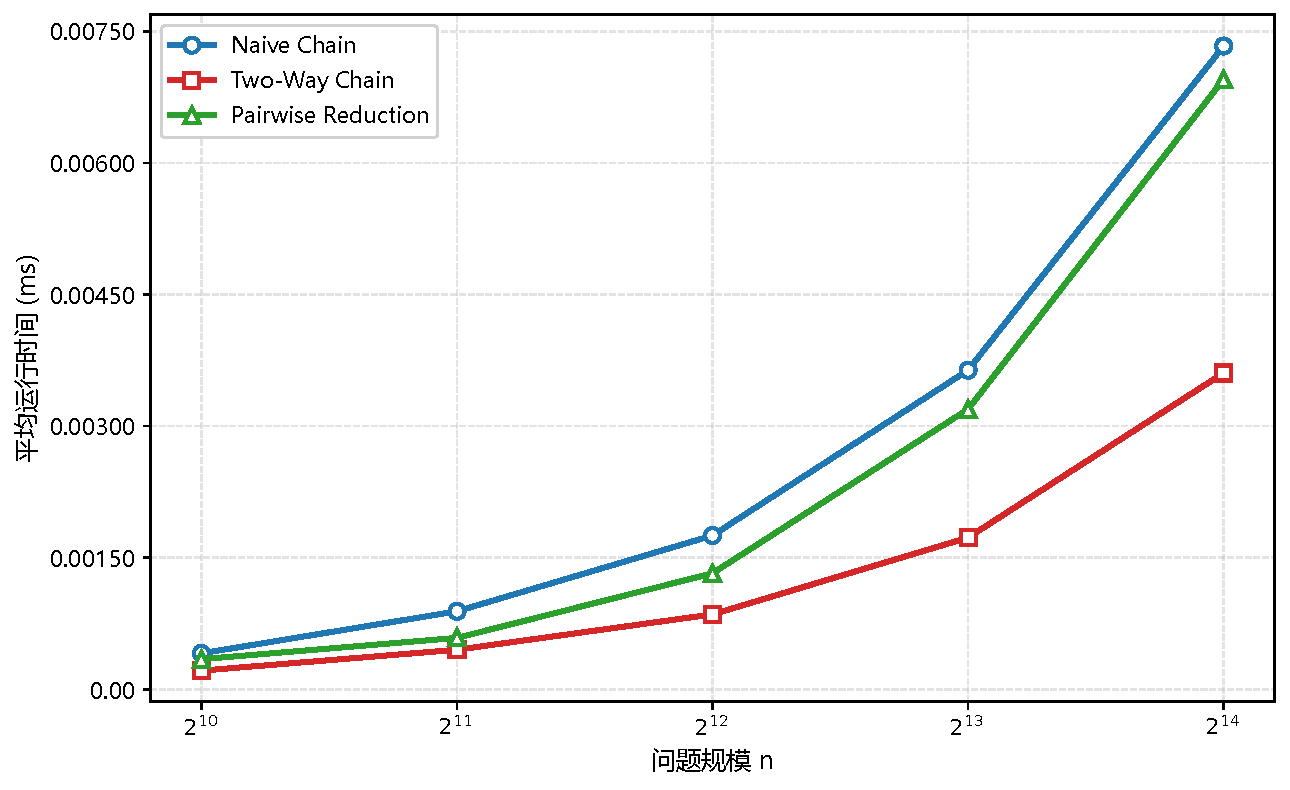
\includegraphics[width=0.88\textwidth]{fig/n_number_sum_runtime_curve.pdf}
    \caption{\(n\) 个数求和运行时间折线图}
    \label{fig:sum-runtime}
\end{figure}

在该实验中，三种算法都能够得到一致的求和结果，但由于其数据依赖关系和中间数据处理方式不同，运行时间存在显著差异。其中，两路链式累加整体最优，说明通过增加独立累加链可以有效提升指令级并行度。
至于为何递归算法未能超过两路链式累加，主要原因会在后文进行剖析。

\subsection{profiling}

\subsubsection{\(n*n\) 矩阵与向量内积}
本次我们对于编译后的程序在VTune上测量其三阶段的cache hit/miss和cpu time、CPI。理论上，平凡算法的热点应集中在按列访问的内层循环中，并且会出现更明显的缓存失配；优化算法则由于按行顺序访问矩阵，cache 行为应明显优于平凡算法。
\begin{figure}[H]
    \centering
    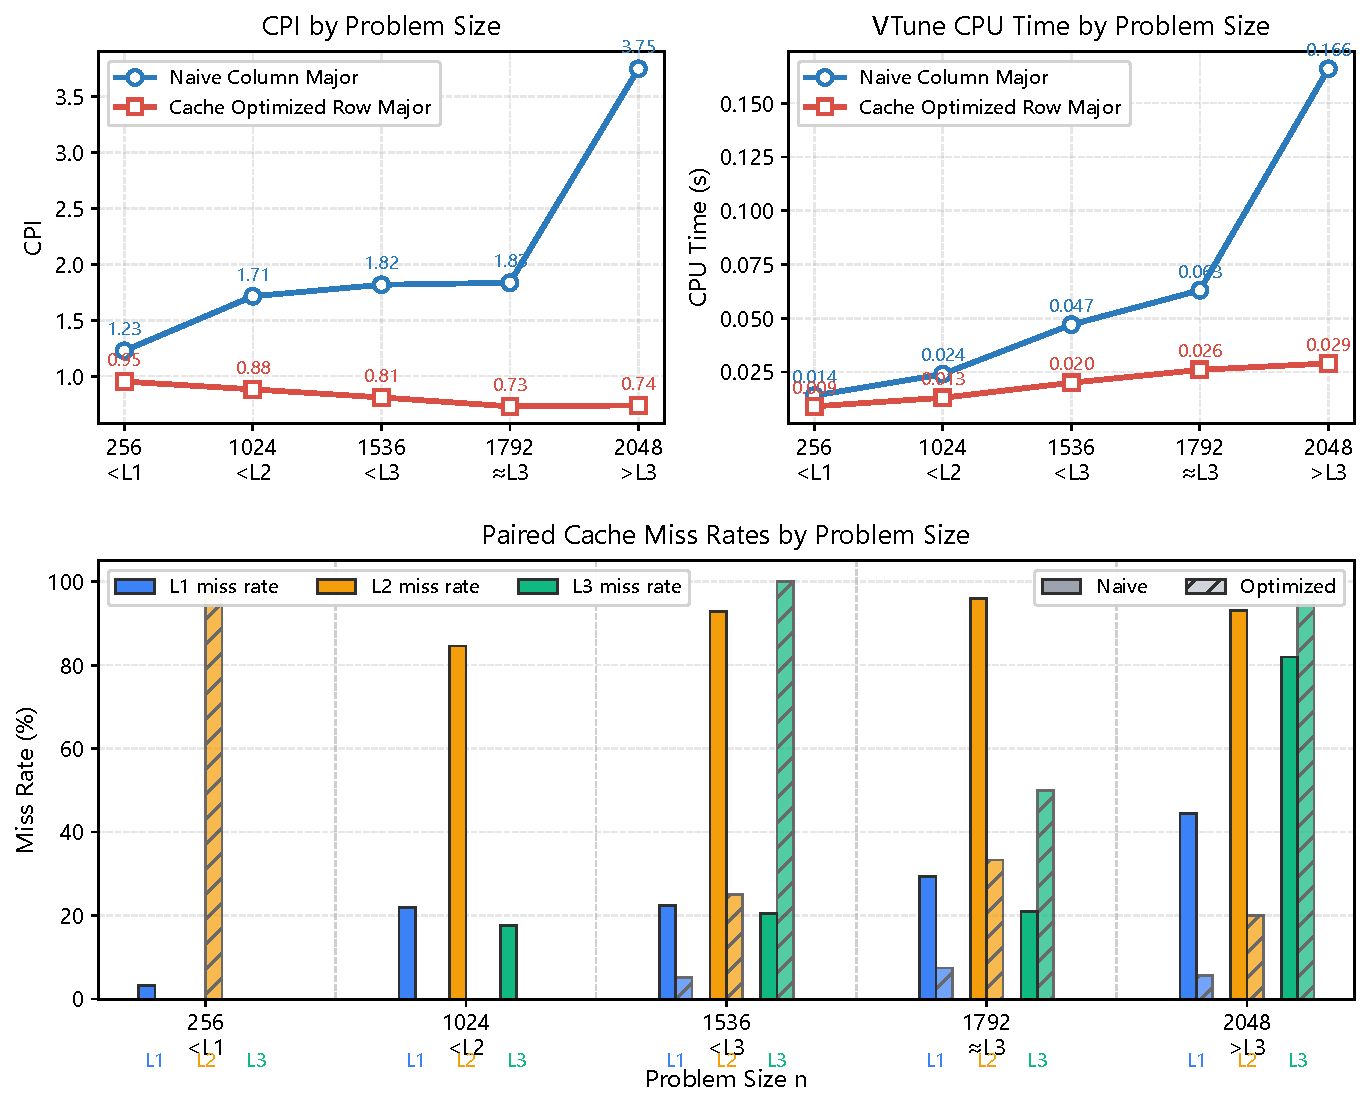
\includegraphics[width=0.70\textwidth]{fig/matrix_cache_cpi_miss_bar.pdf}
    \caption{矩阵与向量内积多规模 profiling 指标图}
    \label{fig:cpi_miss}
\end{figure}

\begin{table}[H]
    \centering
    \small
    \setlength{\tabcolsep}{4.2pt}
    \renewcommand{\arraystretch}{1.20}
    \resizebox{0.99\textwidth}{!}{
    \begin{tabular}{cccccccc}
        \toprule
        \multirow{2}{*}{规模 \(n\)} & \multirow{2}{*}{cache阶段} & \multirow{2}{*}{版本} & \multirow{2}{*}{CPI} & \multicolumn{3}{c}{Cache Miss / Hit} & \multirow{2}{*}{\shortstack{CPU Time\\(s)}} \\
        \cmidrule(lr){5-7}
         &  &  &  & L1 & L2 & L3 &  \\
        \midrule
        \multirow{2}{*}{256}  & \multirow{2}{*}{$<\mathrm{L1}$} & 平凡算法 & 1.227 & 400,006 / 12,000,036 & 0 / 0 & 0 / 0 & 0.014 \\
                              &                                   & 优化算法 & 0.952 & 0 / 6,000,018 & 200,042 / 0 & 0 / 0 & 0.009 \\
        \midrule
        \multirow{2}{*}{1024} & \multirow{2}{*}{$<\mathrm{L2}$} & 平凡算法 & 1.714 & 2,800,042 / 10,000,030 & 2,200,462 / 400,006 & 600,252 / 2,800,588 & 0.024 \\
                              &                                   & 优化算法 & 0.882 & 0 / 8,000,024 & 0 / 400,006 & 0 / 0 & 0.013 \\
        \midrule
        \multirow{2}{*}{1536} & \multirow{2}{*}{$<\mathrm{L3}$} & 平凡算法 & 1.817 & 5,200,078 / 18,000,054 & 5,201,092 / 400,006 & 1,500,630 / 5,801,218 & 0.047 \\
                              &                                   & 优化算法 & 0.810 & 1,200,018 / 22,000,066 & 400,084 / 1,200,018 & 200,084 / 0 & 0.020 \\
        \midrule
        \multirow{2}{*}{1792} & \multirow{2}{*}{$\approx \mathrm{L3}$} & 平凡算法 & 1.835 & 10,800,162 / 26,000,078 & 9,401,974 / 400,006 & 1,700,714 / 6,401,344 & 0.063 \\
                              &                                          & 优化算法 & 0.730 & 800,012 / 10,000,030 & 200,042 / 400,006 & 200,084 / 200,042 & 0.026 \\
        \midrule
        \multirow{2}{*}{2048} & \multirow{2}{*}{$>\mathrm{L3}$} & 平凡算法 & 3.747 & 11,200,168 / 14,000,042 & 10,802,268 / 800,012 & 10,004,200 / 2,200,462 & 0.166 \\
                              &                                   & 优化算法 & 0.739 & 1,200,018 / 20,000,060 & 200,042 / 800,012 & 400,168 / 0 & 0.029 \\
        \bottomrule
    \end{tabular}}
    \caption{矩阵与向量内积多规模 profiling 结果记录表}
\end{table}

具体的结果分析将在后文中结果分析部分展开。

\subsubsection{\(n\) 个数求和}


对于求和实验，本文采用 VTune 的 \texttt{Hotspots} 与 \texttt{Microarchitecture Exploration} 分析类型，重点关注热点函数、执行指令数（Instructions Retired）、时钟周期数（Clockticks）、CPI 以及 CPU time 等指标。平凡链式累加通常会因为单条累加依赖链较长而限制指令级并行；两路链式累加有望在保持较低实现成本的同时显著提升吞吐；递归算法则可能在热点中表现出额外的数组复制和多轮规约开销。

\begin{table}[H]
    \centering
    \small
    \setlength{\tabcolsep}{6pt}
    \renewcommand{\arraystretch}{1.18}
    \resizebox{0.98\textwidth}{!}{
    \begin{tabular}{>{\centering\arraybackslash}p{1.8cm}
                    >{\centering\arraybackslash}p{3.6cm}
                    >{\centering\arraybackslash}p{2.5cm}
                    >{\centering\arraybackslash}p{2.2cm}
                    >{\centering\arraybackslash}p{1.7cm}
                    >{\centering\arraybackslash}p{2.0cm}}
        \toprule
        版本 & 热点函数 & \shortstack{Instructions\\Retired} & Clockticks & \shortstack{CPI\\Rate} & \shortstack{CPU Time\\(ms)} \\
        \midrule
        平凡链式 & \texttt{naiveChainSum} & $4.20\times 10^7$ & $3.64\times 10^7$ & 0.867 & 7.991 \\
        两路链式 & \texttt{twoWayChainSum} & $3.92\times 10^7$ & $1.68\times 10^7$ & 0.429 & 3.995 \\
        递归算法 & \texttt{pairwiseReductionSum} & $1.12\times 10^8$ & $1.96\times 10^7$ & 0.175 & 6.992 \\
        \bottomrule
    \end{tabular}}
    \caption{\(n\) 个数求和 profiling 结果记录表}
\end{table}
\begin{figure}[H]
    \centering
    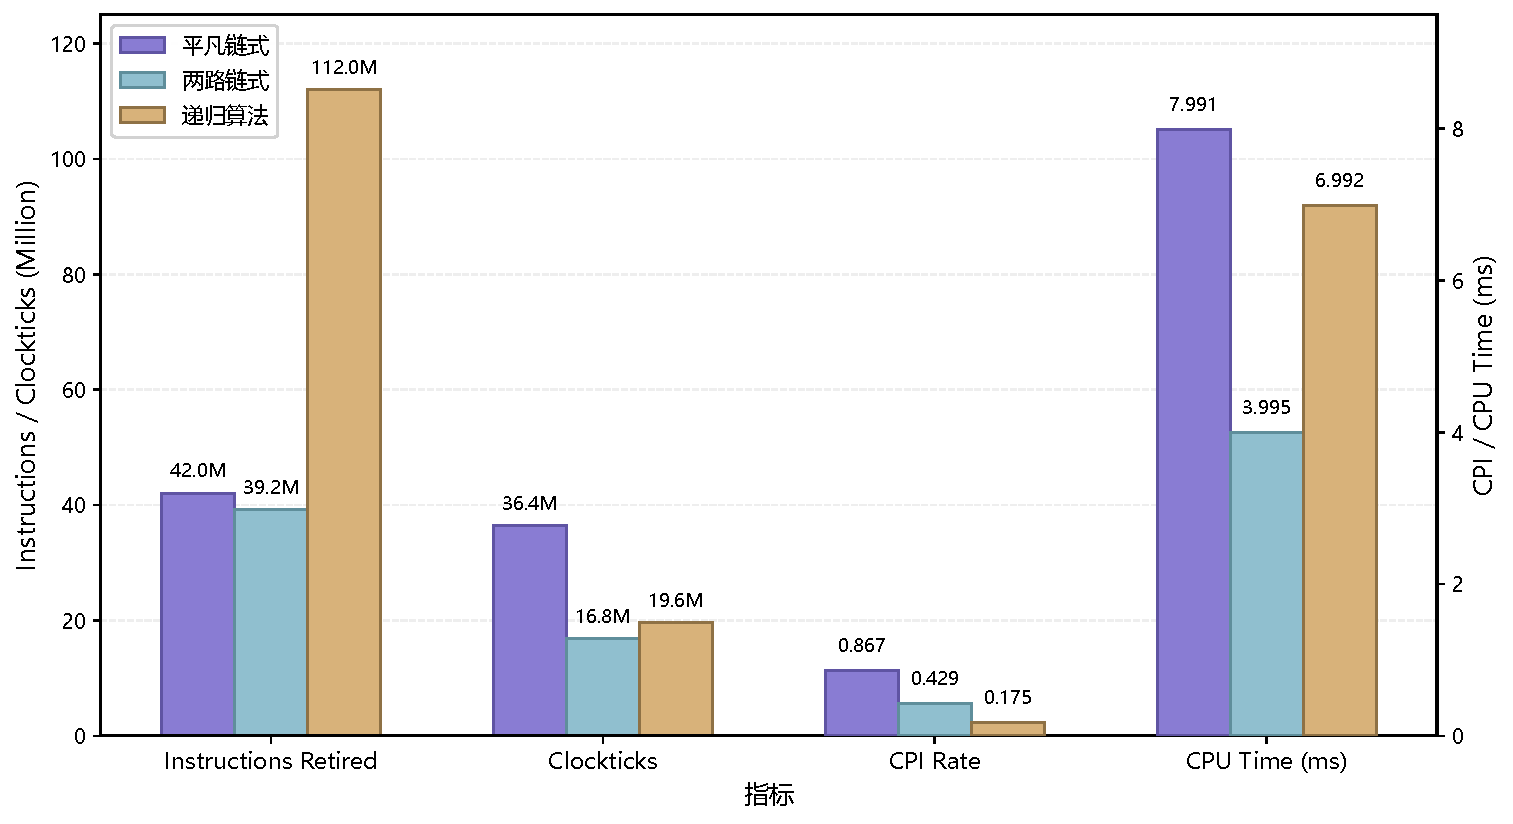
\includegraphics[width=0.72\textwidth]{fig/n_number_sum_profile_bar.pdf}
    \caption{n个数求和 profiling结果图例}
    \label{fig:sum_profile}
\vspace{-0.4em}
\end{figure}

\subsection{结果分析}

\subsubsection{\(n*n\) 矩阵与向量内积}

从表 \ref{tab:matrix-runtime} 和图 \ref{fig:matrix-runtime} 可以看出，矩阵与向量内积的性能变化与 cache 容量阶段高度相关。当 \(n=256\) 时，矩阵仅为 0.50 MiB，仍处在“未充满 L1”阶段，平凡算法与优化算法分别为 0.032270 ms 和 0.020948 ms，加速比只有 1.54 倍，说明此时工作集较小，访存模式差异尚未被层次存储结构充分放大。增大到 \(n=1024\) 后，矩阵达到 8.00 MiB，虽然尚未充满给出的 L2 总容量，但平凡算法时间已升至 3.844896 ms，而按行访问的优化算法仅为 0.310954 ms，加速比迅速增至 12.36 倍。这说明性能拐点并不一定严格出现在“总 cache 容量被完全占满”的位置，而是会更早地受到实际可用 cache 空间、cache line 利用率和硬件预取效果的共同影响。对平凡算法而言，按列访问在行主序存储下属于典型跨步访存，相邻两次访问相隔 \(n\) 个元素，空间局部性很差，很多 cache line 只用到少量数据就被替换；而优化算法按行顺序扫描矩阵，访问连续、预取友好，且单个 \texttt{a[row]} 在一整行中可重复使用，因此随着规模增大，两者差距被迅速拉开。

一个看起来略有“反常”的现象是：加速比并未随规模单调增加，而是在 \(n=1024\) 取得 12.36 倍后，到了 \(n=1536\) 和 \(n=1792\) 反而回落到 7.75 倍和 8.34 倍，直到 \(n=2048\) 才再次跃升到 23.00 倍。这并不说明优化失效，而是因为 \(1536\) 和 \(1792\) 这两个点已经分别进入“超出 L2、逼近 L3”和“基本充满 L3”阶段，优化算法自身也开始更多依赖更低层 cache，故其运行时间由 0.310954 ms 增至 1.481136 ms 和 1.888080 ms；只是它的增长仍明显慢于平凡算法。当规模继续扩大到 \(n=2048\) 时，32.00 MiB 的矩阵已明显溢出 24 MiB L3，平凡算法时间骤增到 53.424360 ms，而优化算法仅为 2.322430 ms，此时 cache 不友好访问所带来的代价被彻底放大，因而出现了最显著的性能分化。profiling 结果与这一结论一致：平凡算法的 CPI 随规模上升由 1.227 增至 3.747，而优化算法基本稳定在 0.73--0.95；在 \(n=2048\) 时，平凡算法的 L1/L2/L3 miss rate 分别达到 44.4\%、93.1\% 和 82.0\%，而优化算法对应仅约为 5.7\%、20.0\% 和 100.0\%。这里优化算法的 L3 miss rate 看起来偏高，\(n=256\) 时甚至还出现了 L2 miss rate 为 100\% 的情况，但这类数值的分母都很小，反映的是“少量真正落到更低层的访问多为冷启动或流式失配”，不能简单理解为整体访存质量很差。综合运行时间与 profiling 可以认为，本实验的主瓶颈并不在乘加次数本身，而在于访存顺序是否顺应 cache 层次结构；按行访问优化的本质，就是把更多访问留在更高层 cache 中完成。


\subsubsection{\(n\) 个数求和}
从表 \ref{tab:sum-runtime} 和图 \ref{fig:sum-runtime} 可以看出，三种求和算法的运行时间都随 \(n\) 近似线性增长，但两路链式累加始终最优，相比平凡链式累加稳定获得约 1.92--2.10 倍加速。这一结果与超标量处理器的执行特点一致：平凡链式累加只有一个累加器，\texttt{sum += x[i]} 之间形成单条长依赖链，后一条加法必须等待前一条完成；而两路链式累加把累加过程拆为 \texttt{sum1} 和 \texttt{sum2} 两条独立链，在几乎不增加额外工作量的前提下提升了指令级并行度。又由于本实验数组规模仅为 8 KiB 到 128 KiB，访问方式始终是顺序扫描，数据大多可以停留在 cache 中，因此影响性能的主要因素不是 cache miss，而是依赖链是否限制了流水线吞吐。也正因为两路链式只比平凡算法多出极少量收尾开销，所以它在所有规模下都表现得最稳定。

递归算法的结果更有代表性：从依赖图看，它构成的是规约树，理论依赖深度约为 \(\log_2 n\)，似乎应当优于链式累加；但本实验实现的是\textbf{单线程、标量、迭代式} pairwise reduction，每次都要先把原数组复制到 \texttt{work}，再进行多轮规约并不断写回中间结果。于是它虽然缩短了单条依赖路径，却显著增加了总工作量。profiling 结果正好说明了这一点：\texttt{pairwiseReductionSum} 函数的 CPI 只有 0.175，低于两路链式累加的 0.429，说明单条指令并不“难执行”；但它的 Instructions Retired 却达到 \(1.12\times 10^8\)，约为两路链式累加 \(3.92\times 10^7\) 的 2.86 倍，因此总 CPU time 仍为 6.992 ms，明显高于后者的 3.995 ms。换言之，递归的问题不是“流水线没跑起来”，而是“为了得到结果做了太多额外事情”。这也解释了为什么它的曲线没有两路链式累加好看：在 \(n=1024\) 到 \(n=2048\) 时，它还能凭借较短依赖链略微优于平凡链式；但随着规模继续增大，多轮遍历和中间结果写回的代价不断累积，其优势逐步被吞掉，到 \(n=16384\) 时仅比平凡链式快约 5\%。因此，在当前单线程 CPU 场景下，最有效的优化并不是单纯追求“理论上更浅的规约树”，而是像两路链式那样，用很低的实现代价打破依赖链；递归更适合在多线程并行规约、SIMD 向量化或树形归并场景下发挥优势。

\section{进阶要求}

\subsection{循环展开优化}

\subsubsection{算法设计}
在基础实验之上，可以继续对核心循环进行循环展开（loop unrolling）优化，以进一步减少循环控制开销并提升处理器吞吐率。针对本实验中的两个问题，可以采用如下思路。
\begin{enumerate}[label=\arabic*.]
    \item 对矩阵与向量内积的按行访问版本，将内层循环按 4 或 8 个元素展开，使一次循环迭代中完成多次乘加操作，从而减少分支与索引更新次数。
    \item 对 \(n\) 个数求和的两路链式累加版本继续展开，例如扩展为 4 路甚至 8 路累加器，进一步增强独立加法链数量，为超标量发射和编译器自动向量化创造条件。
\end{enumerate}

可参考如下伪代码。
\begin{lstlisting}[caption={循环展开优化示意代码}]
// 以 4 路链式累加为例
sum0 = sum1 = sum2 = sum3 = 0;
for (i = 0; i + 3 < n; i += 4) {
    sum0 += a[i];
    sum1 += a[i + 1];
    sum2 += a[i + 2];
    sum3 += a[i + 3];
}
sum = sum0 + sum1 + sum2 + sum3;
\end{lstlisting}

\subsubsection{性能测试}
本节建议在基础实验的相同规模下，增加循环展开版本的独立测试结果，并使用与前文一致的 CSV 导出和折线图展示方式，以便和原始实现直接对比。由于当前仓库中尚未加入循环展开版本的可执行程序，故本节先给出表格模板，待后续补充实测数据。

\begin{table}[H]
    \centering
    \begin{tabular}{cccccc}
        \toprule
        问题类型 & 规模 \(n\) & 原算法（ms） & 展开后（ms） & 加速比 & 备注 \\
        \midrule
        矩阵与向量内积 & 【待填】 & 【待填】 & 【待填】 & 【待填】 & 【待填】 \\
        \(n\) 个数求和 & 【待填】 & 【待填】 & 【待填】 & 【待填】 & 【待填】 \\
        \bottomrule
    \end{tabular}
    \caption{循环展开优化性能测试记录表（待补充）}
\end{table}

\subsubsection{profiling}
建议对循环展开前后的程序再次进行 VTune 分析，重点比较指令退休数量、前端开销以及后端停顿占比的变化，以验证循环展开是否真的减小了循环控制成本，并观察编译器是否在展开基础上进一步做了自动向量化。

\placeholder{【此处插入循环展开优化前后 profiling 对比截图】}

\subsubsection{与原算法对比}
与原算法相比，循环展开优化理论上应具有如下优势：
\begin{enumerate}[label=\arabic*.]
    \item 减少循环分支判断和计数器更新次数，降低控制开销；
    \item 增加同一基本块内的独立运算数量，使处理器更容易挖掘指令级并行；
    \item 在某些场景下为编译器自动向量化提供更好的条件。
\end{enumerate}
但循环展开也可能带来代码体积增加、寄存器压力上升等问题，因此最终效果仍需以实际测试和 profiling 数据为准。\textbf{【待补充：结合后续实测数据填写最终结论】}

\subsection{其他可选进阶优化（待补充）}
除循环展开外，本实验还可以进一步从以下几个方向扩展：
\begin{enumerate}[label=\arabic*.]
    \item 使用 SSE/AVX 等 SIMD 指令实现向量化；
    \item 对比不同编译优化级别（如 \texttt{-O0}、\texttt{-O2}、\texttt{-O3}）对性能的影响；
    \item 分析不同求和顺序对浮点结果误差的影响；
    \item 结合 Godbolt 查看关键循环的汇编代码生成情况。
\end{enumerate}
本节可根据课程进度或个人实验完成情况继续补充，当前先保留为扩展接口。

\section{实验总结和思考}

\subsection{异同对比}
本次两个基础实验都围绕“算法实现与 CPU 架构特性的关系”展开，但二者所体现的重点不同。矩阵与向量内积实验主要反映存储层次结构的重要性：核心差异不在算术操作次数，而在于访问矩阵时是否遵循了内存连续布局；\(n\) 个数求和实验则主要体现指令级并行的重要性：核心差异不在访存模式，而在于是否打破了单条累加依赖链，让处理器能够同时推进更多独立指令。

二者的共同点在于：都不能只从“算法步骤数”出发评价性能，还必须结合具体处理器的 cache、流水线、超标量发射等硬件特性进行分析。也正因为如此，性能测试和 profiling 不能相互替代，前者告诉我们“快了多少”，后者帮助我们理解“为什么会快”。

\subsection{总结和思考}
通过本次实验，我更加直观地认识到“相同数学结果，不同实现方式可能对应完全不同的实际性能”这一事实。对于矩阵与向量内积问题，只是改变访问顺序就能带来数量级上的性能差异；对于求和问题，看似简单的累加操作也会因为依赖链组织方式不同而表现出明显不同的执行效率。这说明在并行与高性能程序设计中，理解底层硬件结构并围绕其特性组织代码，是实现性能优化的关键。

后续若继续完善本实验，建议重点补充以下内容：一是完成循环展开版本的独立实现与测试；二是结合 VTune 的具体数据，将 cache miss、热点函数、停顿来源与前文的性能曲线进行一一对应；三是进一步尝试 SIMD 向量化与编译器优化级别对比，从而形成更完整的 CPU 架构相关优化实验链条。\textbf{【此处也可补充个人在实验过程中的问题、改进思路与心得体会】}

\end{document}









